\documentclass[letterpaper,11pt]{article}
\usepackage[english]{babel}
\usepackage[utf8]{inputenc}
\usepackage[nottoc]{tocbibind}
\usepackage[margin=1.25in]{geometry}
\usepackage[activate={true,nocompatibility},final,
			tracking=true,kerning=true,spacing=true,
			factor=1100,stretch=10,shrink=10]{microtype}

\usepackage{amsmath,apacite,graphicx,wrapfig,setspace,tikz,pgfplots,booktabs,titlesec,fixltx2e,float}
\usepackage[justification=centering]{caption}
\usetikzlibrary{matrix,arrows,calc,3d,fit,patterns}
\frenchspacing
\setcounter{secnumdepth}{4}
\titleformat{\paragraph}
{\normalfont\normalsize\bfseries}{\theparagraph}{1em}{}
\titlespacing*{\paragraph}
{0pt}{3.25ex plus 1ex minus .2ex}{1.5ex plus .2ex}

\title{A Universal Robot Control System using Reinforcement Learning with Limited Feedback}

\author{Joshua Gruenstein \and Michael Truell}

\begin{document}

\maketitle

% 100-200 words

\begin{abstract}

A robot control system was developed that could be taught tasks through reinforcement learning.
The system, nicknamed “Fido”, was designed to be universal regardless of inputs and outputs, robot kinematics, and processing capability.
In addition, Fido was built to learn with limited feedback, allowing humans to train Fido in a minimal amount of time.
This was achieved through the training of artificial neural networks with a wire-fitted interpolator following the Q-learning reinforcement learning algorithm and an intelligent action selection policy that utilizes a probabilistic approach to exploration.
Functionality was first tested and evaluated in simulation.
Next, hardware implementations of differing kinematics, sensors, and central processors were constructed.
Fido successfully converged on all given tasks in simulation and in hardware within very few learning iterations while maintaining impressively low latency, demonstrating its potential as a comprehensive robot control system.

\end{abstract}


\pagebreak

\section{Intro}

The most prevalent control system used in mobile robotics is a procedurally programmed expert system (Biggs \& MacDonald, 2003).
 Such systems use linear conditional logic in order to emulate a desired behavior.
 However, such systems are limited in numerous respects.
 First, they can only perform the specific task for which they were programmed to accomplish; the entire software must be rewritten in order to change the target task.
 Second, they rely on a knowledge of the inputs and outputs to the robot (such as sensors and motor control) in order to function.
 The purpose of Fido was to solve both of these problems, allowing a universal general control system for robots that can be trained on tasks using reinforcement learning.

We chose to approach this problem with artificial neural networks; function appropriators modeled after nature with the capability to take in a large number of inputs to produce an output.
 Neural networks are commonly used to solve tasks that are challenging using traditional rule-based programming, making them perfect for our task.
 The control system was named Fido for the name's connotations to training an intelligent organism.


\section{Background}

The human brain is composed of billions of neurons, interconnected electrically excitable cells that form the basis of intelligence.
Each neuron has dendrites that receive electrical signals from other neurons.
If the sum of these electrical signals is greater than a certain threshold value, the neuron fires, propagating a voltage down its axon and out of its synapses.
These synapses can be considered the output of the neuron and are themselves connected to the dendrites of other neurons.
The interconnections of these neurons form a massive network, where a huge number of inputs are processed in parallel to a set of outputs.
The purpose of artificial neural networks is to simulate the mathematical properties of these neurons in order to approximate complex functions.

\subsection{Single Artificial Neuron}

\begin{figure}[ht]
	\centering
	\def\layersep{2.5cm}
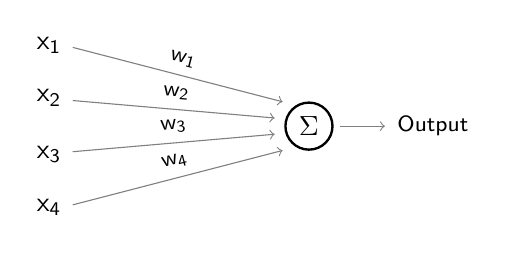
\begin{tikzpicture}[font=\sffamily,shorten >=1pt,->,draw=black!50, node distance=\layersep]
    \tikzstyle{every pin edge}=[<-,shorten <=1pt]
    \tikzstyle{neuron}=[circle,line width=0.3mm,draw=black,minimum size=17pt,inner sep=0pt]
    \tikzstyle{annot} = [text width=4em, text centered]


    \draw[->] (-3,1) -- (-.3,.3) node[sloped,midway,above] {\footnotesize w\textsubscript{1}} node[left=3cm,above=.5cm]{x\textsubscript{1}};

    \draw[->] (-3,0.325) -- (-.4,.1) node[sloped,midway,above] {\footnotesize w\textsubscript{2}} node[left=2.9cm,above=.03cm]{x\textsubscript{2}};
 
    \draw[->] (-3,-.325) -- (-.4,-.1) node[sloped,midway,above] {\footnotesize w\textsubscript{3}} node[left=2.9cm,below=.03cm]{x\textsubscript{3}};
 
    \draw[->] (-3,-1) -- (-.3,-.3) node[sloped,midway,above] {\footnotesize w\textsubscript{4}} node[left=3cm,below=.5cm]{x\textsubscript{4}};
    
    \node[neuron] (0,0) {$\Sigma$};

    \draw[->] (.4,0) -- (1,0) node[right] {\footnotesize Output};
\end{tikzpicture}
	\caption{Single Neuron Diagram}
\end{figure}

An artificial neuron is simply a mathematical model of a biological neuron, and therefore its functionality is very similar.
Each artificial neuron has multiple inputs, each one the output of a different neuron.
In addition, each neuron has a weight for each input, a bias term, an activation function, and one output.
The output of one neuron becomes the input of other connected neurons.
The output of a neuron is expressed mathematically for $n$ inputs $x$ and weights $w$, a bias term $b$, and activation function $O(x)$:

\begin{align*}
	\text{activation} = \sum_{i=0}^{n}x_i w_i + b\\
	\text{output} = O(\text{activation})
	\,.
\end{align*}

A weight is a positive or negative number that governs the impact of of its respective input on the neuron's single output.
The bias term is a number added to the summation of weights and inputs, allowing us to make affine transformations on the domain of the activation function.

In biologically inspired neurons, the activation function is a binary step function.
If the activation function's input is less than a certain threshold, the output is zero.
If it is greater than the threshold, the output is one.
However, a binary output can be somewhat limiting for many applications of neural networks.
Many of Fido's outputs are gradient rather than binary; as an example, Fido can set the brightness of a light-emitting diode.
Because of this, alternate activation functions with gradient outputs are used.
One such function is the sigmoid function.
In addition to being continuous, the sigmoid function is differentiable, allowing the network to be trained, and nonlinear, allowing the network to model a broader range of functions.
The sigmoid function is expressed as such:

\begin{equation}
	O(a) = \cfrac{1}{1+e^{-\frac{a}{p}}}
	\,,
\end{equation}

\noindent for each output $O$, activation $a$, and constant $p$.
The sigmoid activation function can also be graphed as below.

\begin{figure}[ht]
	\centering
	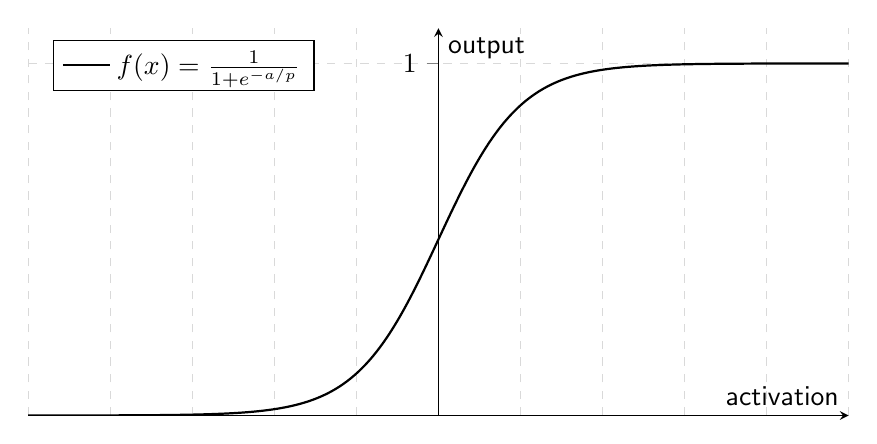
\begin{tikzpicture}[font=\sffamily]
    \begin{axis}[
    	legend pos=north west,
        axis x line=middle,
        axis y line=middle,
        grid = major,
        width=12cm,
        height=6.5cm,
        grid style={dashed, gray!30},
        xmin=-1,xmax= 1,ymin= 0,ymax= 1.1,
        xlabel=activation,ylabel=output,
        tick align=outside,
        ytick={1},
        xmajorticks=false,
        enlargelimits=false]
      \addplot[domain=-1:1,black,thick,samples=500] {1/(1+exp(-10*x))}; 
      \addlegendentry{$f(x)=\frac{1}{1+e^{-a/p}}$}
    \end{axis} 
\end{tikzpicture}
	\caption{Sigmoid Function Graph}
\end{figure}

\subsection{Feed-forward Neural Network}

A traditional method of arranging artificial neurons in a neural network is called a feed-forward network.
Neurons are connected as previously described: the output of each neuron is connected to one of the inputs of another neuron.
These neurons are organized into layers, as described in Figure \ref{fig:feedforward}.

\begin{figure}[ht]
	\centering
	\def\layersep{2.5cm}
\begin{tikzpicture}[shorten >=1pt,->,draw=black!50, node distance=\layersep,font=\sffamily]
    \tikzstyle{every pin edge}=[<-,shorten <=1pt]
    \tikzstyle{neuron}=[circle,line width=0.3mm,draw=black,minimum size=17pt,inner sep=0pt]
    \tikzstyle{annot} = [text width=4em, text centered]

    \foreach \name / \y in {1,...,4}
        \node[neuron, pin=left:Input \y] (I-\name) at (0,-\y) {};

    \foreach \name / \y in {1,...,5}
        \path[yshift=0.5cm]
            node[neuron] (H-\name) at (\layersep,-\y cm) {};

    \node[neuron,pin={[pin edge={->}]right:Output}, right of=H-3] (O) {};

    \foreach \source in {1,...,4}
        \foreach \dest in {1,...,5}
            \path (I-\source) edge (H-\dest);

    \foreach \source in {1,...,5}
        \path (H-\source) edge (O);

    %\draw[->] (5,-2.9) -- (5,-5) -- (1,-5) -- (1,-4.5);
    %\node (1,-4.5) {Error back propagation}

    \node[annot,above of=H-1, node distance=1cm] (hl) {Hidden layer};
    \node[annot,left of=hl] {Input layer};
    \node[annot,right of=hl] {Output layer};
\end{tikzpicture}
	\caption{Single Output Feed-forward Network}
	\label{fig:feedforward}
\end{figure}

The output of each neuron in a layer becomes an input of every neuron in the next layer.
In this way, the original inputs of the neural network are ``fed forward'' layer by layer, starting from the first layer (the input layer), passing through any number of middle layers (hidden layers), and ending with the last layer (the output layer).
The outputs of the neurons in the output layer are the outputs of the whole network.

Fido is a feed-forward network.
Sensor inputs such as light and sound are sent into the input layer.
The outputs of output layer neurons are used to change the speed of Fido's motors, the color of Fido's LEDs, and the sound of Fido's buzzers.

\subsection{Backpropagation}

Supervised learning is the modification of the weights of a neural network's neurons in order to reach a specific output from a specific set of inputs.
One such method of adjusting neural networks weights is called back propagation \cite{werbos}.

\begin{figure}[ht]
	\centering
	\def\layersep{2.5cm}
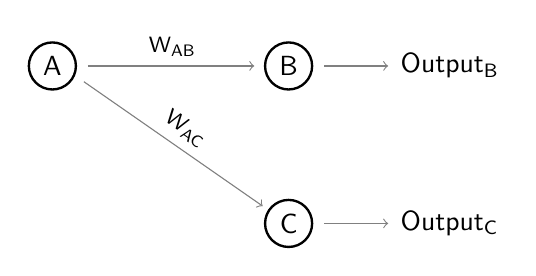
\begin{tikzpicture}[font=\sffamily,shorten >=1pt,->,draw=black!50, node distance=\layersep]
    \tikzstyle{every pin edge}=[<-,shorten <=1pt]
    \tikzstyle{neuron}=[circle,line width=0.3mm,draw=black,minimum size=17pt,inner sep=0pt]
    \tikzstyle{annot} = [text width=4em, text centered]

    \draw[->] (.45,0) -- (2.6,0) node[sloped,midway,above] {\footnotesize W\textsubscript{AB}};
    \draw[->] (.4,-.2) -- (2.7,-1.8) node[sloped,midway,above] {\footnotesize W\textsubscript{AC}};

    \draw[->] (3.45,0) -- (4.3,0) node[right=0cm]{Output\textsubscript{B}};
    \draw[->] (3.45,-2) -- (4.3,-2) node[right=0cm]{Output\textsubscript{C}};
    
    \node[neuron] at (0,0) {A};
    \node[neuron] at (3,0) {B};
    \node[neuron] at (3,-2) {C};
\end{tikzpicture}
	\caption{Single Branch in a Back Propagation Neural Network}
	\label{fig:backprop}
\end{figure}

Neural networks learning through back propagation are trained through example.
Example inputs (known as training sets) are linked to a particular target output, forming a training pair.
The first step of training is to pass in an arbitrary training set to a neural network with randomly generated weights.
The error $\delta$ for an output neuron is defined as the difference between the actual output and the target output for that training set.
As an example we will use the single connection described in Figure \ref{fig:backprop}.
The neural network in this figure has only an input layer consisting of Neuron $A$ and an output layer consisting of Neurons $A$ and $B$.
$W_{AB}$  and $W_{AC}$ are the weights between the neurons.
We first determine the Neuron $B$ error $\delta_B$ as $\text{Target}_B - \text{Output}_B$.
 Next we modify weight $W_{AB}$ as follows, defining $W_{AB}^{+}$ as the newly trained weight:

\begin{equation}
	W_{AB}^{+} = W_{AB} + (\delta_B \text{Output}_A)\,.
\end{equation}

The same approach could be taken for Neuron $C$.
However, this method cannot calculate an improved weight for hidden layer neurons such as Neuron $A$, as there is no predefined target.
Therefore we must calculate the error of $A$ indirectly by back propagating from the two output layer neurons, for which the error is already known:

\begin{equation}
	\delta_A = W_{AB}\delta_B + W_{AC}\delta_C \,.
\end{equation}

Once the error for Neuron $A$ is obtained, its trained weights can be calculated in the same fashion as done for Neuron $B$.
This pattern can be repeated throughout a larger neural network in order to converge upon the network's target output.

\subsection{Q-Learning}

Reinforcement learning seeks to find the optimal action to be undertaken for a given state through trial and error.
In the context of Fido, an action could be the playing of a note or driving straight forwards, while the state could be the amount of light detected by the robot or how near the robot is to another object.
Once an action is performed, a reward and a new state are given back to the reinforcement learning algorithm.
As actions are performed over time, the reinforcement learning algorithm sharpens its ability to receive reward.

$Q$-Learning \cite{watkins} is a popular reinforcement learning algorithm that works by learning an action-value function $Q$ that takes a state-action pair as an input and outputs the expected utility value of performing that action in that state.
This utility value is know as the $Q$-value.
The $Q$-value is a combination of immediate reward and expected future reward.
Every learning iteration the $Q$-value of an state-action pair is updated as such:

\begin{equation}
	Q(s, a) := Q(s, a)(1 - \alpha) + \alpha(R + \gamma \max Q(s_{t+1}, a))
	\,,
	\label{equ::updateqlearn}
\end{equation}

\noindent
where $a$ is the action carried out, $s$ is the initial state, $R$ is the reward received, and $s_{t+1}$ is the new state.
$\alpha$ is the learning rate of the algorithm.
The learning rate determines the rate of convergence by diminishing or amplifying the changes made to the $Q$-value each learning iteration.
$\gamma$ is the devaluation factor, which determines the weight given to future rewards.
A devaluation factor approaching $\gamma=0$ will force the algorithm to only value immediate reward, while a devaluation factor approaching $\gamma=1$ will make it focused on high long term reward.
A table is used to model the $Q$ function, storing past state-action pairs and each pair's respective $Q$-value.


\section{Learning}

\subsection{Wire-Fitted Q-Learning}

The $Q$-Learning algorithm had to be immediately modified to be able to work in continuous state-action spaces for it to be suitable for Fido.
Conventional $Q$-Learning is discrete.
No relation is made between states or actions, and every action for each state must be performed individually in a noisy feedback system to determine its $Q$-value.
However, Fido will work in a large, continuous state-action spaces where relations made between (state-action, $Q$-value) pairs can drastically reduce the number of learning iterations needed for convergence.
An example of a task that would benefit from continuity is teaching Fido to adjust the speed of its motors based on the intensity of light that the robot detects.
There is an obvious gradient relation between the (state-action, $Q$-value) pairs in this task and with a limited number of $Q$-values known, it is possible to correctly model $Q$.

To accommodate continuous action-spaces, we coupled a wire-fitted moving least squares interpolator with our feed-forward neural network as described in \cite{gaskett}.

Feed-forward neural networks can generalize between states in $Q$-Learning problems with discrete actions as described in \cite{rummery}.
To extend this implementation to a continuous action space, our feed-forward neural network outputs discrete ``wires'' when given a state.
Each wire consists of an action with its respective $Q$-value for the state given to the neural network.
These wires may be interpolated to model $Q$, allowing us to get the $Q$-value of any action performed in a state given as an input to the network.
The interpolator used in Fido is a wire-fitted moving least squares interpolator used in the context of a memory-based learning system \cite{baird}.

The wire-fitting function calculates $Q$-value of an action $\hat{a}$ for a state $s$ given a set of $n$ actions $a$ each with a respective $Q$-value $q$ as such:

\begin{equation}
	Q(a, s) = \cfrac{\sum_{i=0}^{n}\cfrac{q_i}{||\hat{a}-a_i||^2+c(q_{max}-q_i)+k}}{\sum_{i=0}^{n}\cfrac{1}{||\hat{a}-a_i||^2+c(q_{max}-q_i)+k}}
	\,,
\end{equation}

\noindent
where $q_{max}$ is the greatest $Q$-value among the set of $Q$-values $q$, and $k$ is a small value that avoids division by zero.
$c$ is the smoothing factor.
The greater the smoothing factor, the smoother the interpolated function.


Figure \ref{fig::wirefitexample} is an example of interpolation on a set of wires.
The graph shows the value of one-dimensional actions plotted against their respective $Q$-values.
The wire-fitting function has few properties that make it especially suited for Fido.

\begin{figure}[ht]
   \centering
   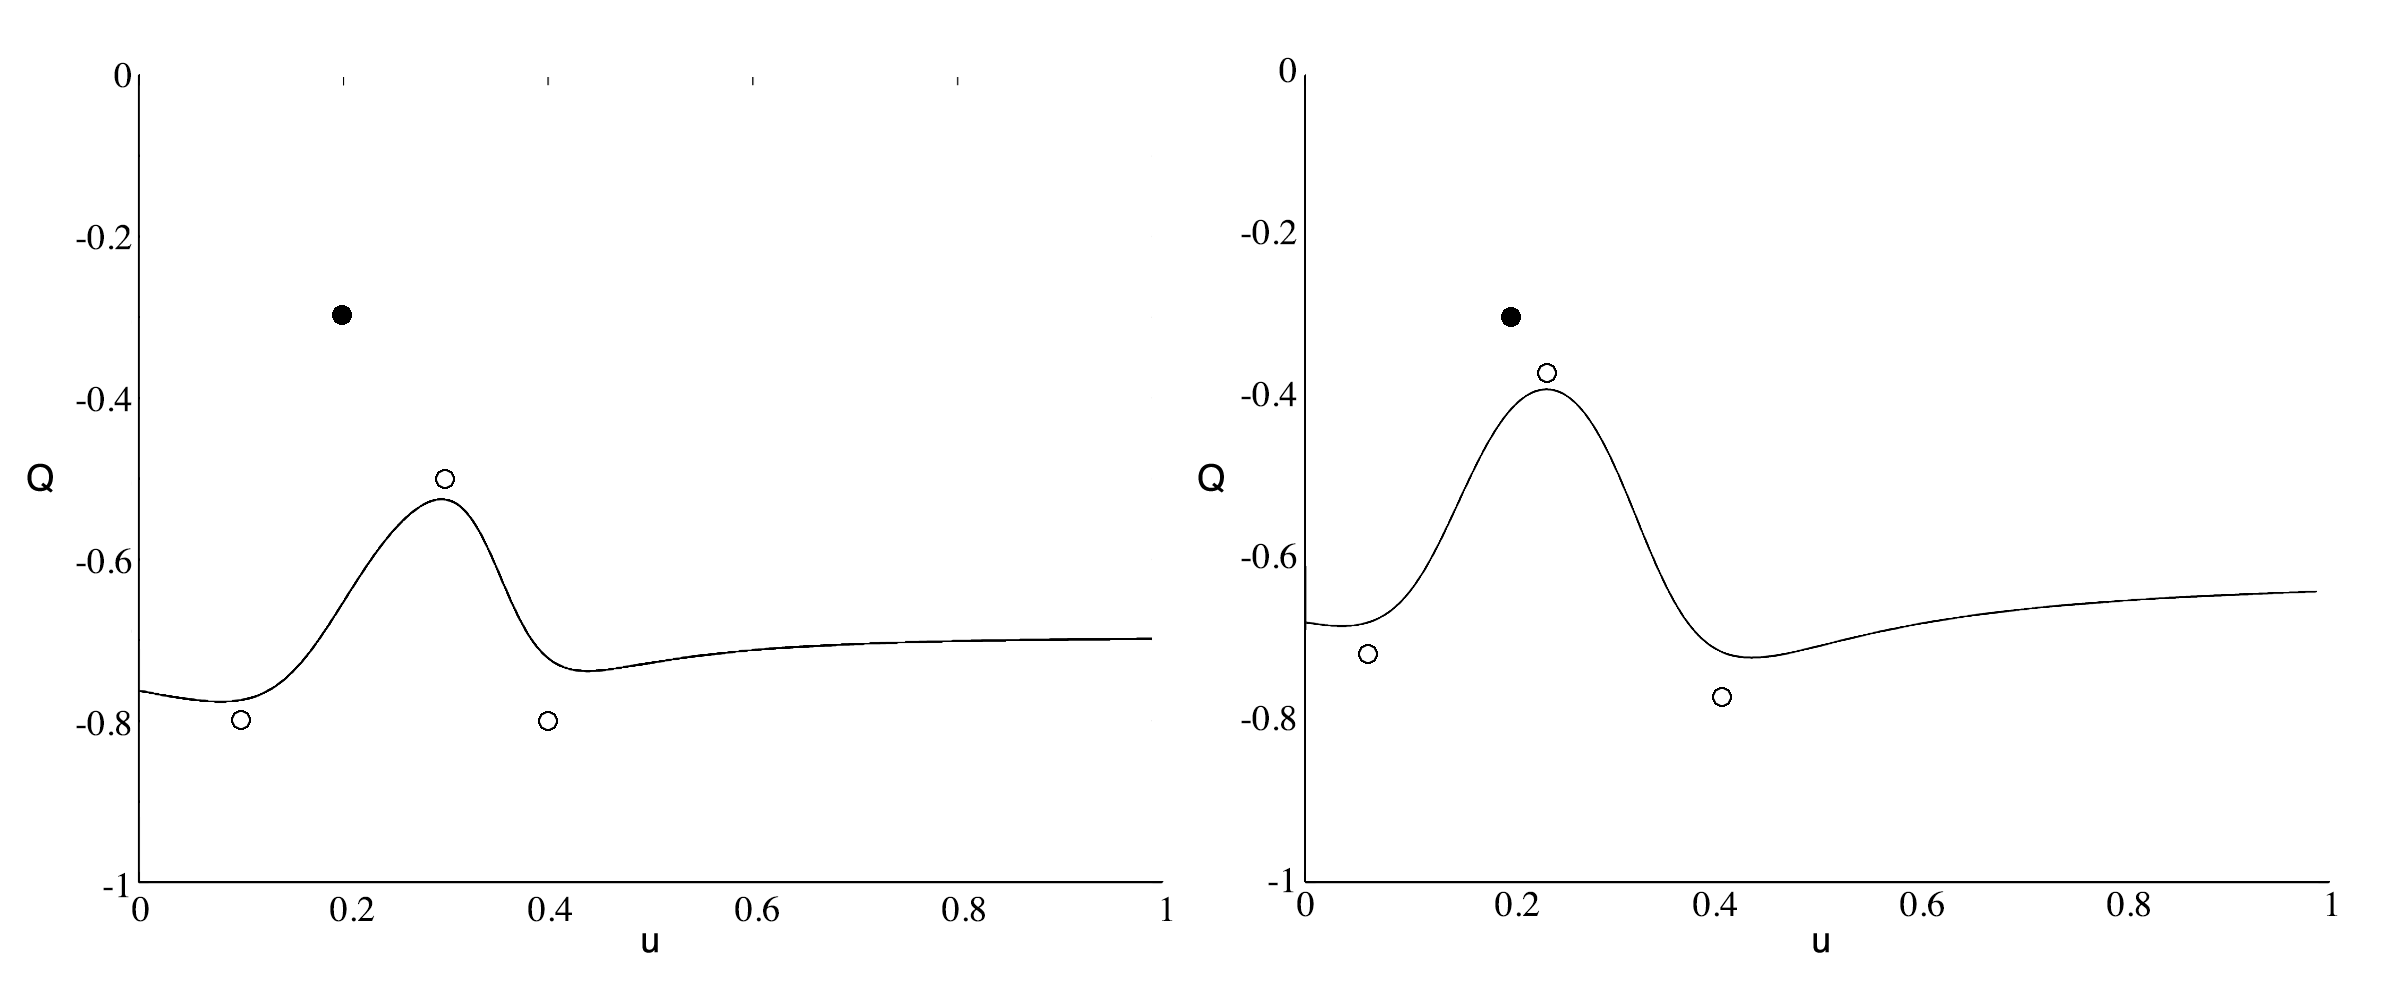
\includegraphics[height=6.5cm]{Figures/WireFit.png}
	\caption{Moving Least Squares Interpolator (adapted from Gaskett, Wettergreen, \& Zelinsky, 1999)}
   \label{fig::wirefitexample}
\end{figure}

Every update to the $Q$-value requires that $q_{max}$ is computed and the action that produces $q_{max}$ is needed for common action selection policies.
As proved in \cite{baird}, the wire with the greatest $Q$-value is the interpolation point with the greatest $Q$-value, therefore $q_{max}$ is the maximum $Q$-value out of the set of wires given to the wire-fitting function.
This makes it extremely computationally cheap to compute $Q$-value, allowing Fido's latency to stay minimal.

The wire-fitting function is derivable.
This allows us to update our wires, and therefore our model of $Q$, using gradient descent.
Gradient descent is an optimization algorithm that looks to find the local minimum of a function by modifying each of its parameters, one by one.
The update function for a parameter is calculated as such:

\begin{equation}
	a = a - \gamma \Delta F(a)
	\,,
	\label{equ::wirefiterrorfunction}
\end{equation}

where $a$ is the parameter to be updated, $\gamma$ is the learning rate, and $\Delta F(a)$ is the partial derivative of the function to be minimized $F$ with respect to $a$.
In the case of Fido, once the reward and new state for an action-state pair is received and an updated $Q$-value $\hat{q}$ is calculated using Equation \ref{equ::updateqlearn}, we are trying to minimize the wire-fitting function's error at predicting $\hat{q}$ when given the wires for Fido's previous state.
This error can be calculated as:

\begin{equation}
	(\hat{q} - q)^2
	\,,
	\label{equ::wirefiterrorfunction}
\end{equation}

\noindent

where $q$ is the old $Q$-value.
Using Equation \ref{equ::wirefiterrorfunction} as our function to be minimized and the partial derivative of the wire-fitting function with respect to each action vector and each q-value, we may compute the partial derivatives of our cost function.
Using these, new wires may be calculated for Fido's previous state using gradient descent.

Fido's neural network may be trained is trained to output these wires using the Adadelta training algorithm. Adadelta is a variant of backpropgation that dynamically adjusts its learning rate to an optimum value, allowing for lower latency. This increases the universality of Fido, since backpropagation's learning rate is task specific.

\subsection{Uncertainty Value}

Fido continuously calculates the "uncertainty" $u$ of its system. Such a value should lower as Fido learns a task and rise if Fido's task changes. This value is useful in adjusting a number hyperparameters that are detailed in the next few sections, such as the exploratory level of the system. After receiving reward and updating its wires using stochastic gradient descent, Fido calculates its uncertainty value as the means squared error between its original set of wires and its newly updated set of wires. In this way, Fido uncertainty value is proportional to the disparity between the current predictions of its model and new information presented to Fido during the current learning iteration.

\subsection{Action Selection}

$Q$-learn requires that actions are selected to be performed.
There are a number of approaches to choosing this action, and each has a large affect on the behavior of the learning implementation.
The most common approach is to simply pick the action with the best $Q$-value for the current state.
However this strategy stifles exploration of the state-action space, increasing the time of convergence on a task, hurting the retrain-ability of the model, and giving a bias towards an actor's starting policy, which is random.
This problem is compounded in the case of Fido due to the large state and action spaces that Fido must explore.
Another common method of action selection is to choose each action randomly for a set number of learning iterations, and then to switch to choosing the action with the highest $Q$-value.
This plan improves upon the first by allowing for a period of exploration, but is not suited for Fido.
During its lifetime, Fido must have the ability to learn new tasks and be retrained by the operator providing feedback, and so, must continuously explore its state space.

Fido selects actions probabilistically using a Boltzmann or soft-max distribution of probability.
The likelihood that an action $\hat{a}$ will be chosen from a set of $n$ actions $a$ for a state $s$ is given as:

\begin{equation}
	p(\hat{a}) = \cfrac{e^{\frac{Q(s, \hat{a})}{T}}}{\sum_{i=0}^{n}e^{\frac{Q(s, a_i)}{T}}}
	\,.
	\label{equ::boltzmann}
\end{equation}

$T$ is the temperature, or exploration level.
As $T$ approaches infinity, a random action is chosen.
As $T$ tends toward 0, the best action is chosen.
Fido keeps $T$ at a constant value around $T \approx 0.15$ throughout its lifetime to encourage occasional, continued exploration.

$T$ is set proportional to Fido's uncertainty value, so that Fido rapidly explores when it is first initialized or is being retrained. This allows Fido to converge on tasks in fewer learning iterations than if $T$ were set as a constant. As Fido learns a task, $T$ will approach 0. This means that Fido will accurately perform a task when sure of its actions, increasing Fido's average reward over other systems.

\subsection{Experience Replay}

As a reinforcement learning system proceeded throughout a problem, the effect of former learning iterations decreases with time as the system updates the parameters of its model to lower its error on new learning iterations. This is wasteful since some iterations will present the system with critical information, such as tagging an unlikely action with high reward.

Fido stores each learning iteration's initial and final states, action, and reward, collectively known as an "experience." Every learning iteration, Fido trains its model on a few past experiences, which are sampled probabilistically according to their age. Weight is given to newer experiences. The number of experiences sampled is proportional to the inverse of Fido's uncertainty value, as past histories will become invalid if the parameters of a problem change. This practice, called "experience replay," lowers the number of learning iterations required for convergence by utilizing all of the information available to Fido.

\subsection{Dynamic Model Architecture}

The optimal size of a neural network is directly related to the complexity of the function that such a neural network has to model. This requires that Fido dynamically size its network, since a constant neural network architecture would never be able to converge on some tasks. Likewise, Fido must dynamically optimize the number of wires outputted by its neural network, since more complicated tasks require a larger number wires to effectively model their action-reward function.

The most accurate method of model architecture optimization would be a brute force search. When using such a method, all the possible permutations of Fido's model within a range would be generated. Each possible model would be trained on a sample of Fido's experiences for a finite number of epochs. The model with the lowest error on the sample of experiences would be selected as Fido's current model.

However, such a method is extraordinarily latent and since Fido needs to be able to run on low power systems, is infeasible. Stochastic gradient descent would be a natural choice for such a search, but the relationship between Fido's error and its model architecture is not easily derivable.

Instead, Fido performs a simultaneous perturbation stochastic approximation to adjust its model architecture. SPSA is gradient descent method designed for discrete systems that requires only two samples of the cost function to compute its derivative. Its update function is similar to \ref{equ::wirefiterrorfunction} and is given as:

\begin{equation}
	u_{n+1} = u_n - a_n\hat{g_n}(u_n)
	\label{equ::spsaupdate}
\end{equation}

\noindent

where $n$ is the current epoch; $u$ is our model parameters, the number of wires and neurons; $a$ is a positive sequence of numbers that approach 0 as $n$ approaches 0; and $\hat{g_n}$ is an estimation of the derivative of the cost function. SPSA defines $\hat{g_n}$ as:

\begin{equation}
	\hat{g_n}(u_n) = \cfrac{J(u_n + c_n\Delta_n)-J(u_n - c_n\Delta_n)}{2c_n(\Delta_n)_i}
	\,.
	\label{equ::spsaderivative}
\end{equation}

\noindent

where $\Delta_n$ is a random perturbation vector and $J$ is the cost function. For Fido, $J$ is the error of the the model $m_n$ that is defined by $u_n$ on a sample of experiences after a period of training.

To optimize the sampling of $J$, Fido creates $m_n$'s neural network by adding and subtracting the Fido's current network since Fido's model at any given time will have a relatively low $J$. Fido subtracts "unimportant" neurons using a pruning algorithm so as to decrease $J(m_n)$. Our pruning algorithm estimates the effect of pruning weight $w_{ij}$ on $J$. This estimate using values recorded during backpropagation or Adadelta and is given as:

\begin{equation}
	\sum_{b=0}^{B}\cfrac{\delta E}{\delta w_{ij}}\Delta w_{ij}(b)\cfrac{w^f_{ij}}{w^f_{ij}-w^i_{ij}}
	\label{equ::sensitivity}
\end{equation}

Neurons whose weights have the smallest impact on $J$ should be pruned.


\section{Implementation}

Fido was implemented in the C++ programming language with minimal use of the standard library.
This was to enable cross-platform functionality, lightweight and speedy performance, and the ability to run on microcontrollers if necessary.
In order to test Fido both a simulation environment and three hardware implementations were constructed and written driver suites for interaction with inputs and outputs.

\subsection{Simulation}

An asynchronous simulator was created using C++ and the SFML graphics library in order to efficiently test Fido's performance on different types of robots.
Multiple inputs were modeled for simulation with outlets for control both by a human operator using sliders and by programmed handlers using a bridge class.
Sensors included a microphone, light sensor, infrared light sensor, inertial measurement unit, and three axes of radio receivers allowing measurement from a radio beacon.
Multiple tasks were trained using both operator input and autonomous ``taskmaster'' programs to regulate positive and negative feedback.


\begin{figure}[H]
	\centering
	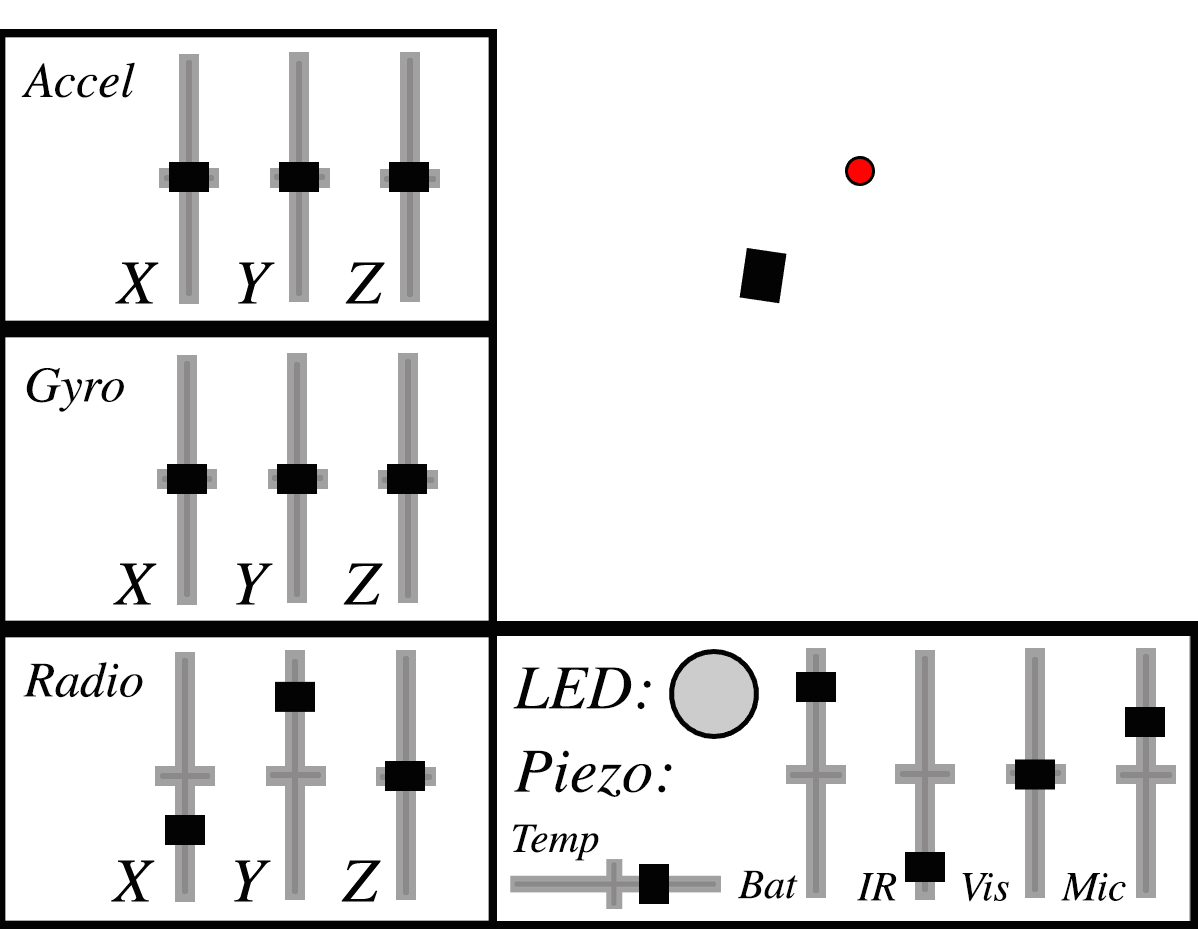
\includegraphics[height=10cm]{Figures/Screenshot.png}
	\caption{Screenshot of the Fido Simulator Graphical User Interface}
\end{figure}

Fido's outputs were chosen similarly.
A buzzer of varying tone and frequency can play sounds and a multicolor LED can be lit to any red-green-blue color combination.
Two motors allow movement using one of two kinematic configurations: differential drive similar to that of a tank, or holonomic control for each axis of movement.
Appropriate kinematics for each model including acceleration and friction were implemented with help from \cite{dudek}.

The black rectangle in the upper right corner of the simulator is the robot, having been moved as part of training.
The red dot near the rectangle is a graphical representation of a radio beacon.
As adjusting sliders to represent the location of a radio beacon relative to the robot would be impractical, we decided to implement a beacon that could be placed and dragged by right clicking on the simulator.
Simulated sensor readings of beacon strength on two axes are gathered using an inverse square law, as applies to radio waves in general.
These readings are then displayed in the sliders and can be manually altered as well.
The radio beacon can be removed by a human operator by pressing the ``p'' key in the simulator environment.
This was especially helpful in the task of training Fido to follow a radio beacon.

\subsection{Hardware Implementations}

Three hardware implementations were next constructed to test Fido's real world trainability, universality, and applicability.
In order to facilitate this, the three robots were designed to have vastly different kinematics and functionality.
The robots, nicknamed ``Thing One,'' ``Thing Two,'' and ``Thing Three,'' all ran on embedded GNU/Linux systems and were trained via a cross-platform mobile application over Wi-Fi.

\subsubsection{Thing One}
\begin{figure}[H]
	\centering
	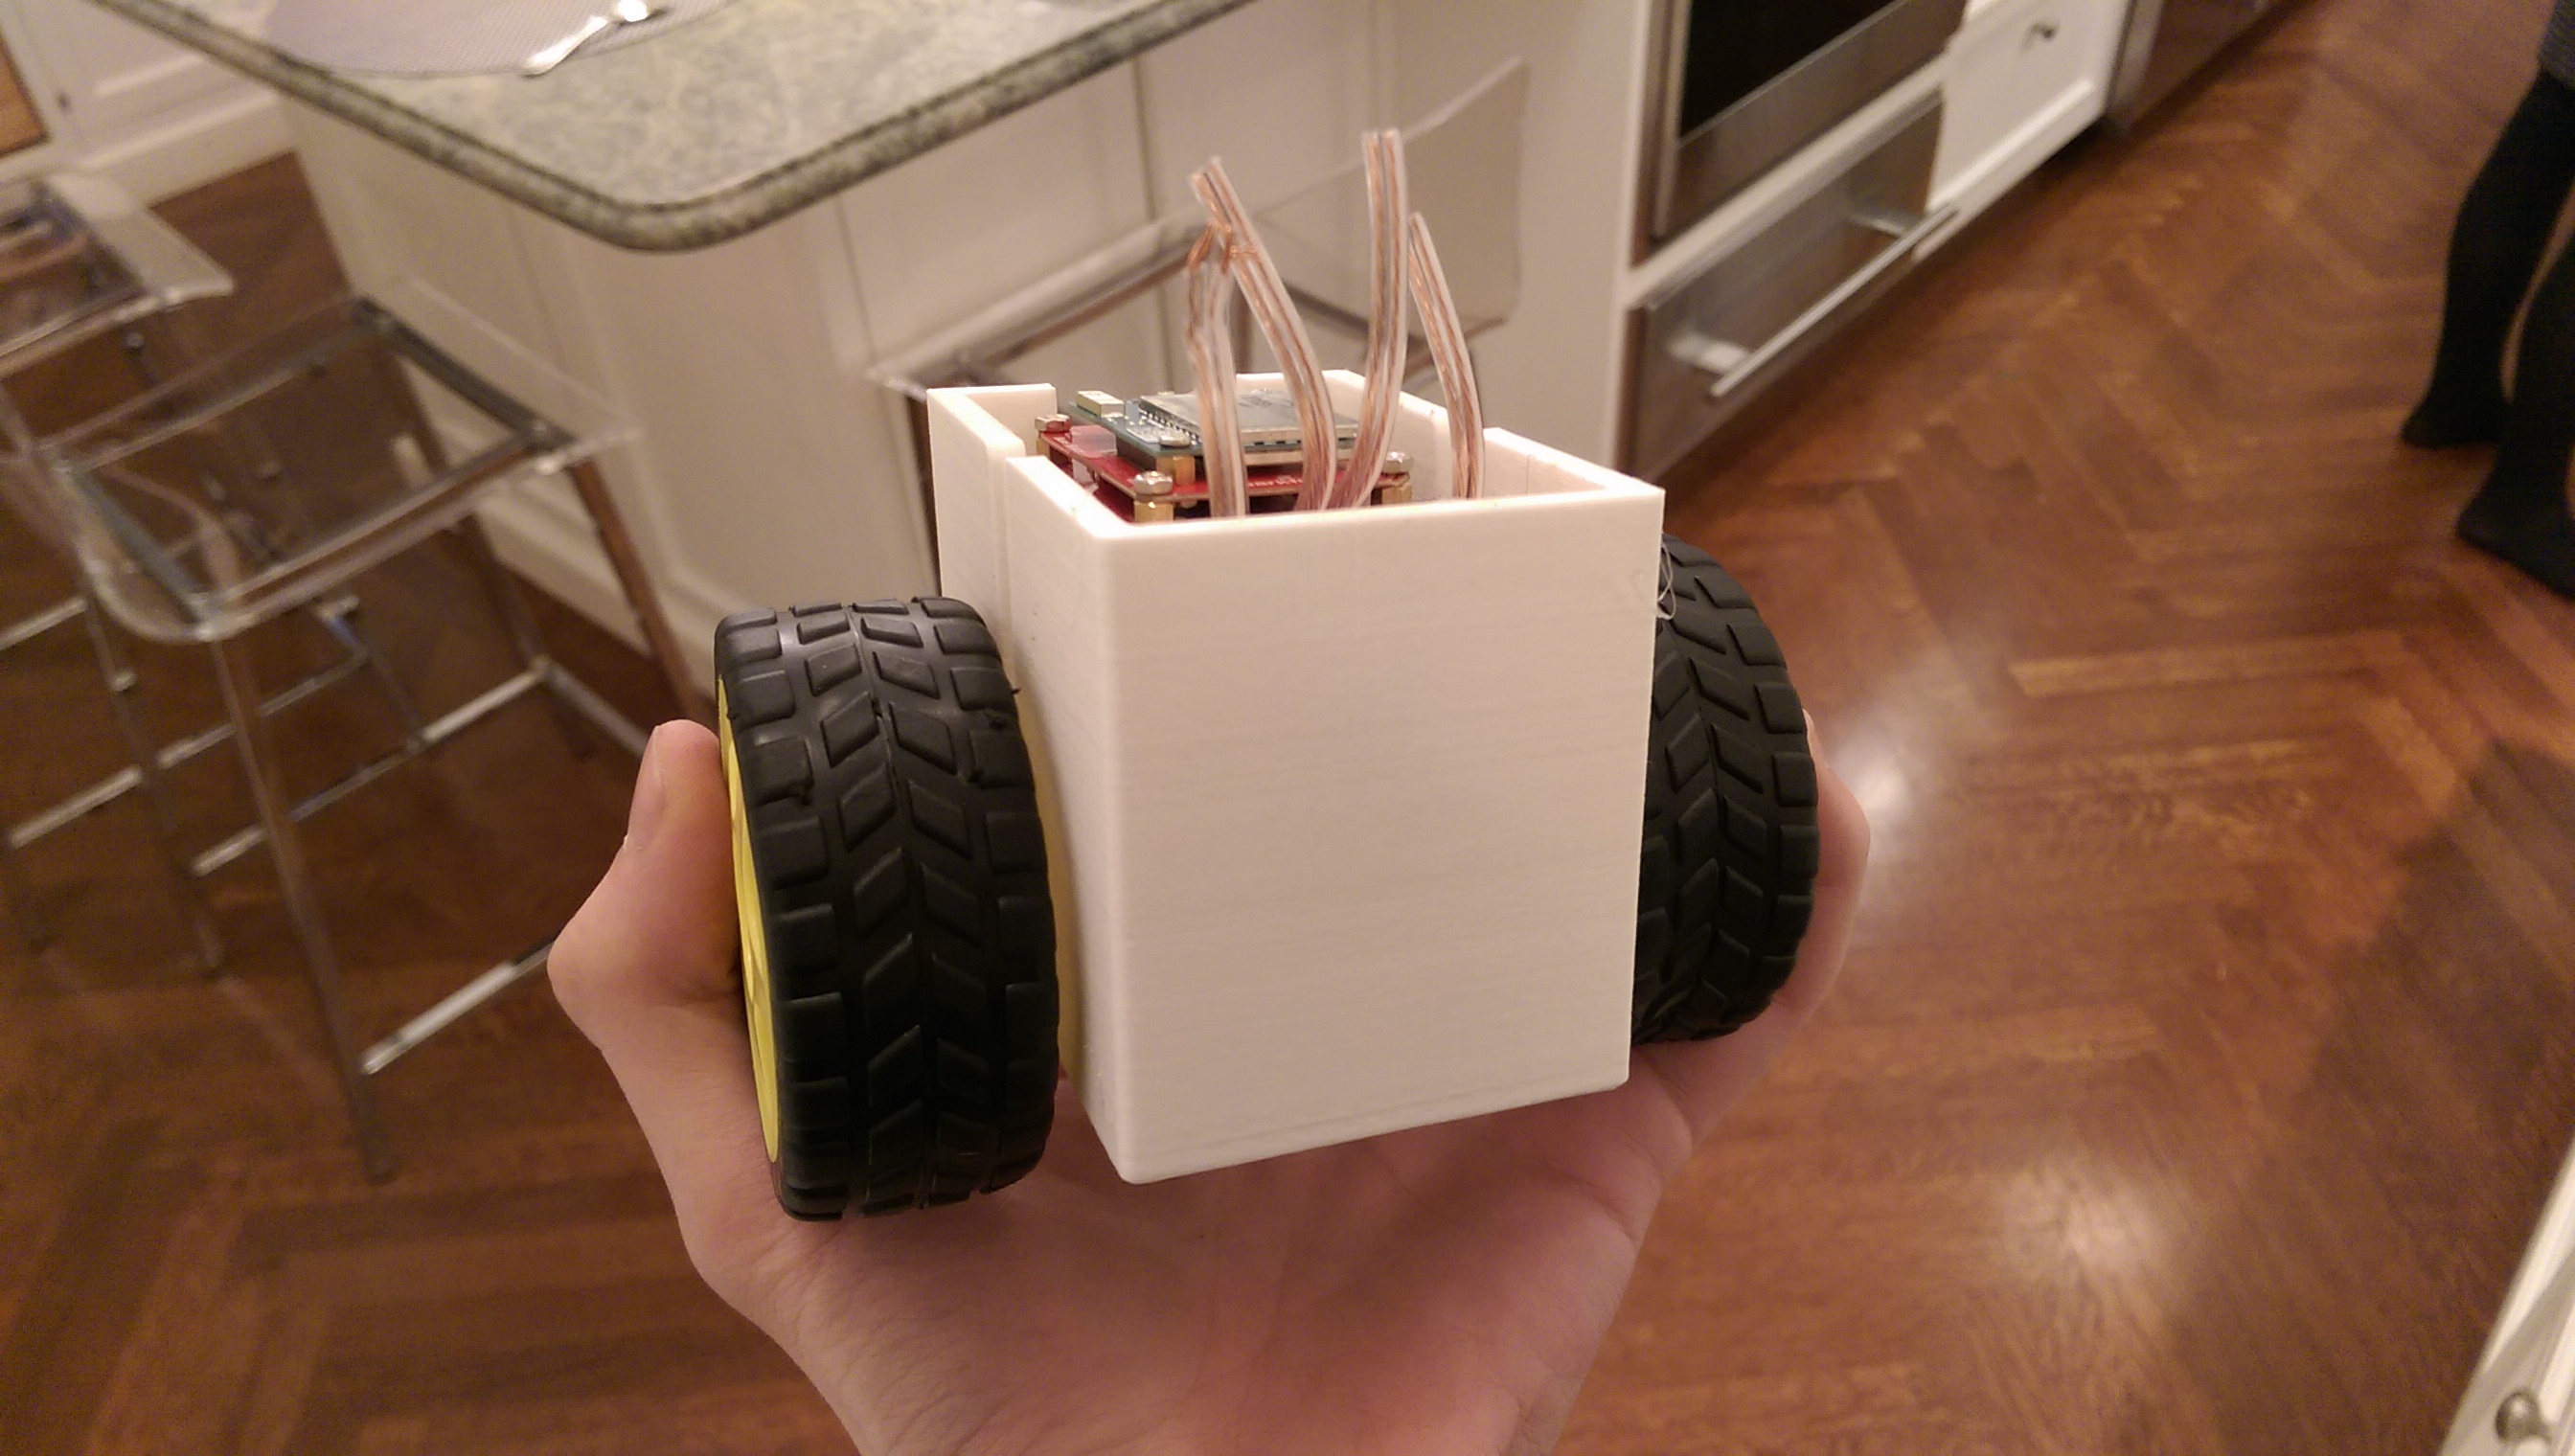
\includegraphics[height=6cm]{Figures/Prototype.jpg}
	\caption{Fido Thing One with Head-Cap Removed}
\end{figure}

The first hardware implementation constructed, nicknamed ``Thing One,'' consisted of an Intel Edison GNU/Linux Single Board Computer, a two-wheeled differential drive system, and a 3D-printed case.
The implementation was given an ambient light sensor, an inertial measurement unit, and a microphone as inputs, with its two motors as outputs.
A differential drive system was chosen due to its standardization in the field, while the Intel Edison was chosen due to its low power consumption and integrated wireless networking capabilites.

\subsubsection{Thing Two}
\begin{figure}
	\centering
	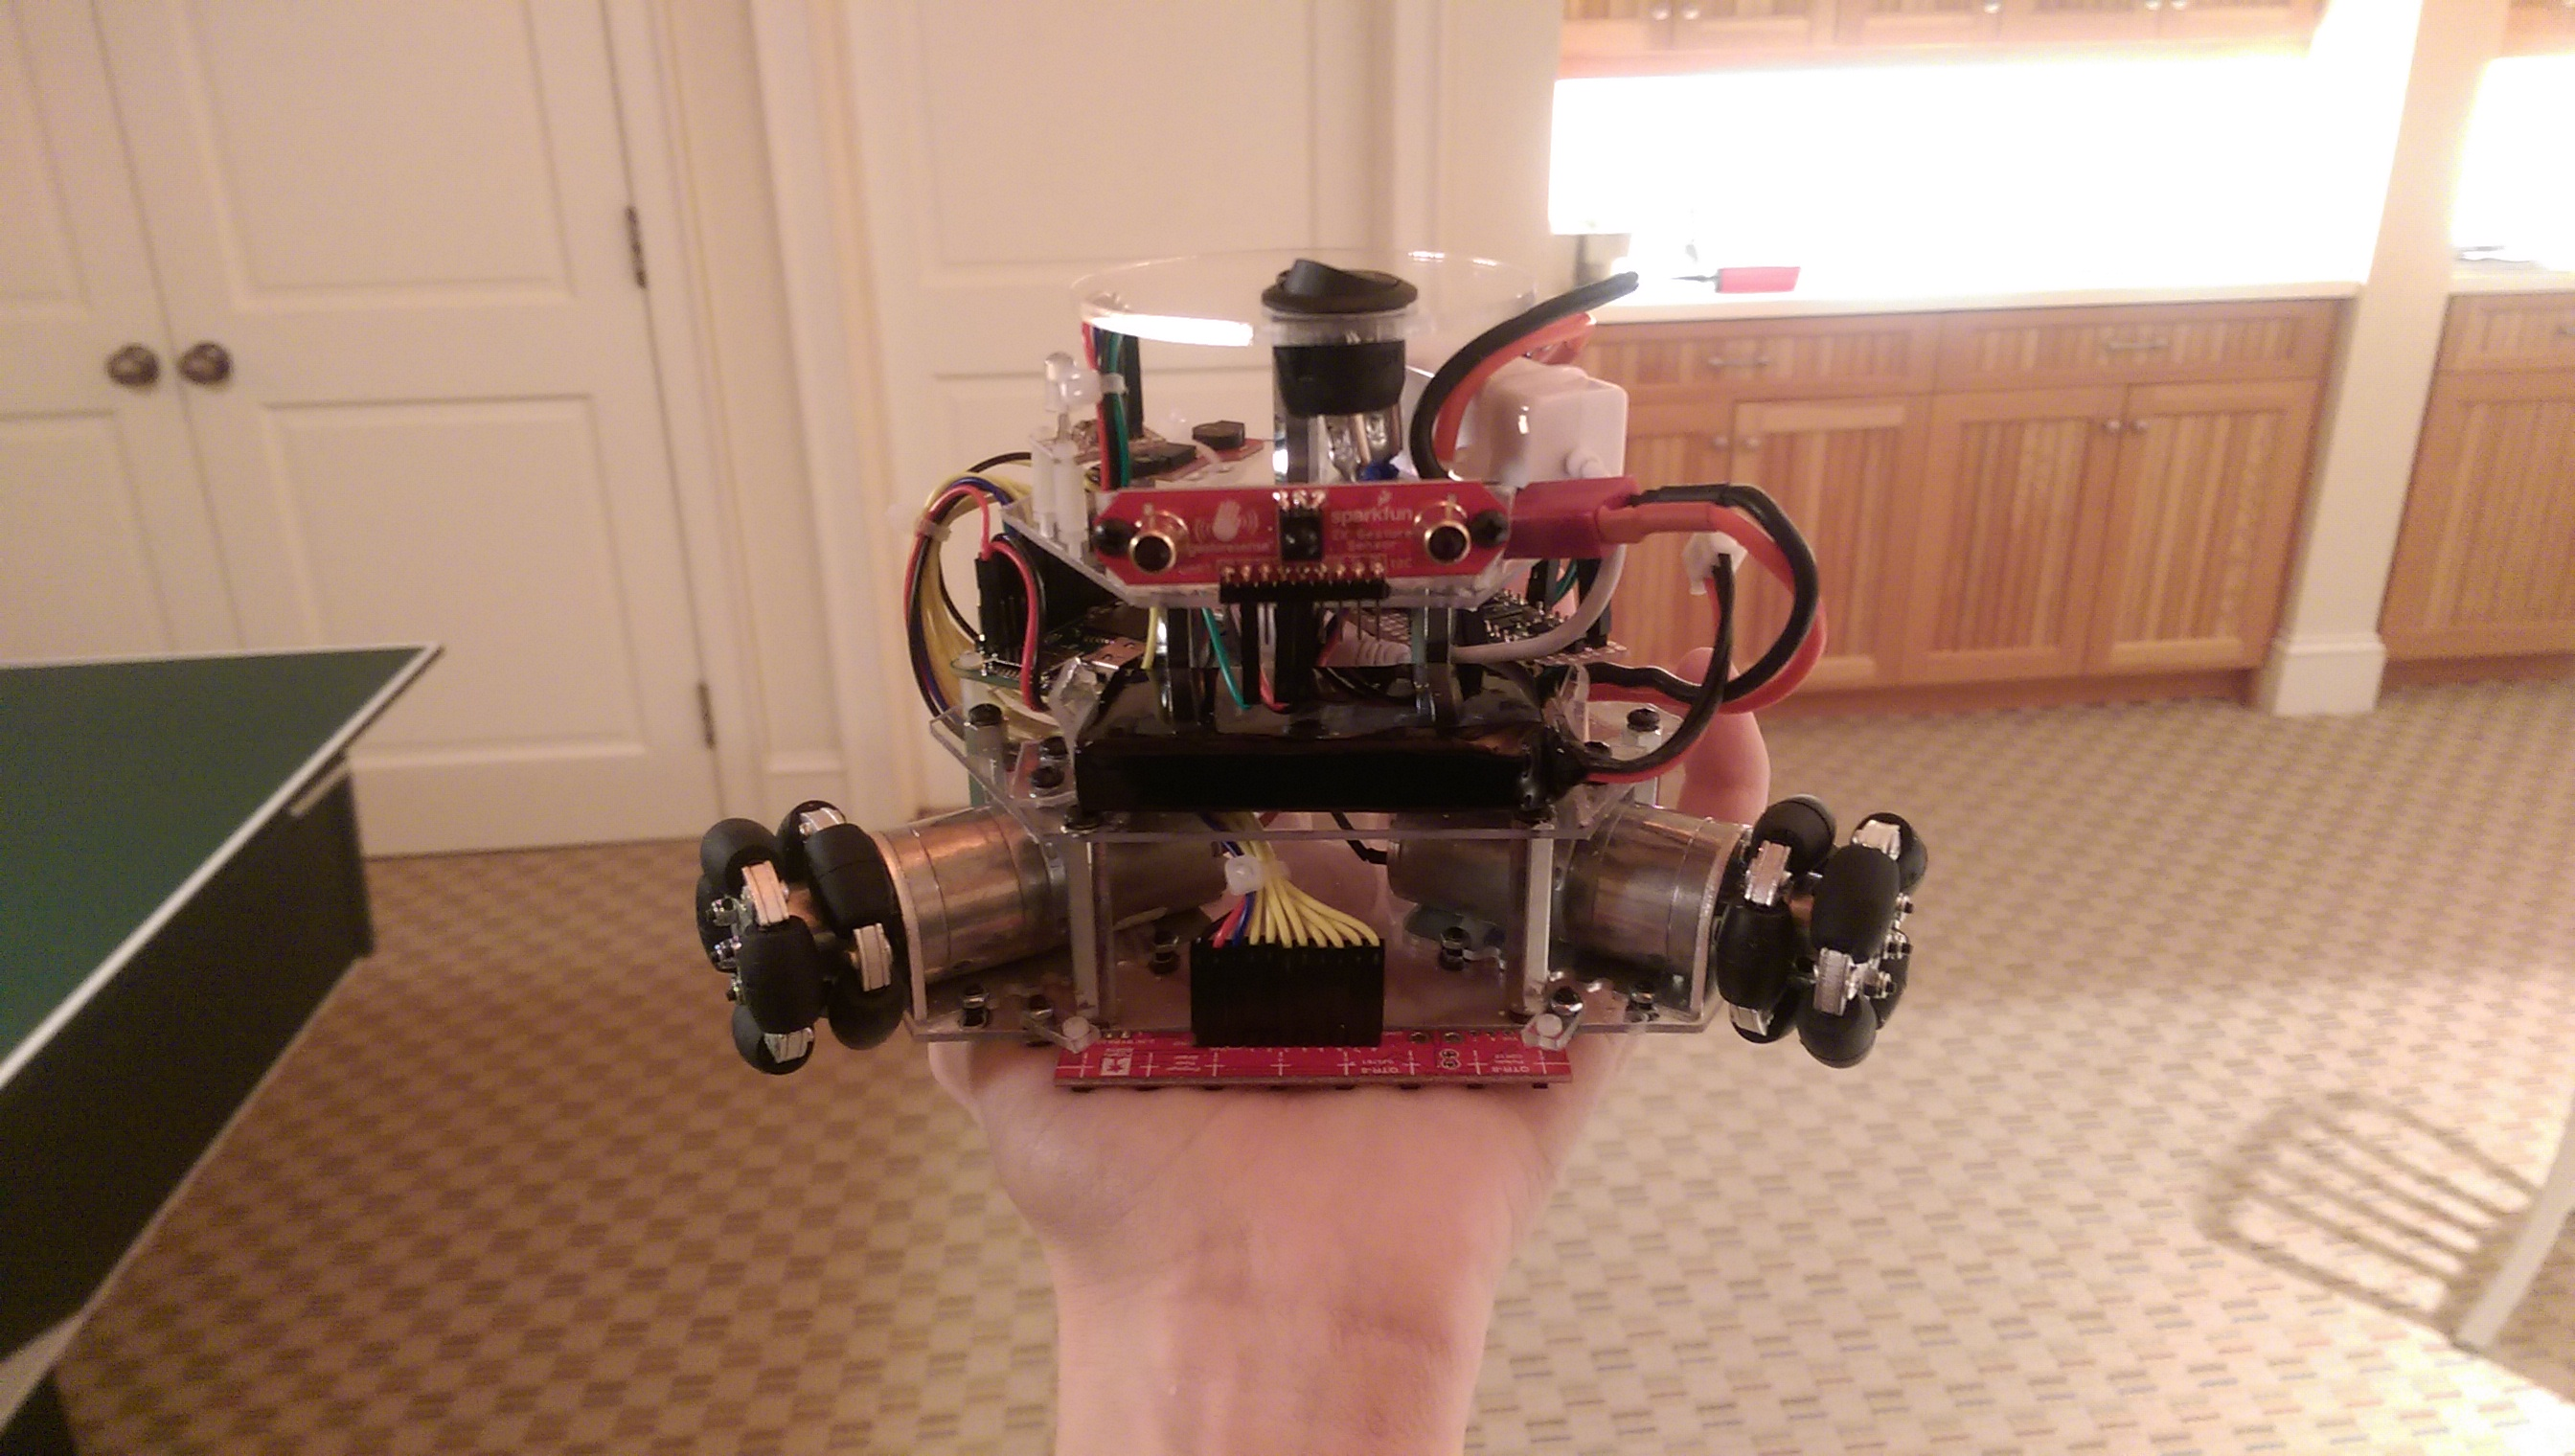
\includegraphics[height=6cm]{Figures/ThingTwo.jpg}
	\caption{Fido Thing Two}
\end{figure}

The second hardware implementation to be constructed was named ``Thing Two,'' and utlized a three 90$^{\circ}$ Swedish wheel holonomic drive system.
This more complex drive system challenged the Fido control system with the advanced kinematics neccesary to manipulate the system in every possible degree of freedom.
The robot was powered by the \$5 Raspberry Pi Zero, demonstrating that Fido could be run on lower cost and power hardware.
The body was cut from 1/8\" polycarbonate and bolted together using hex standoffs to create a tiered structure for mounting various sensors and electronics.
The inputs to the system were a ZX gesture sensor, a line following infrared array, an inertial measurement unit and an ambient RGB color sensor.
The outputs from the system were its three motors, a piezoelectric buzzer, and an RGB light-emitting diode.

\subsubsection{Thing Three}
\begin{figure}
	\centering
	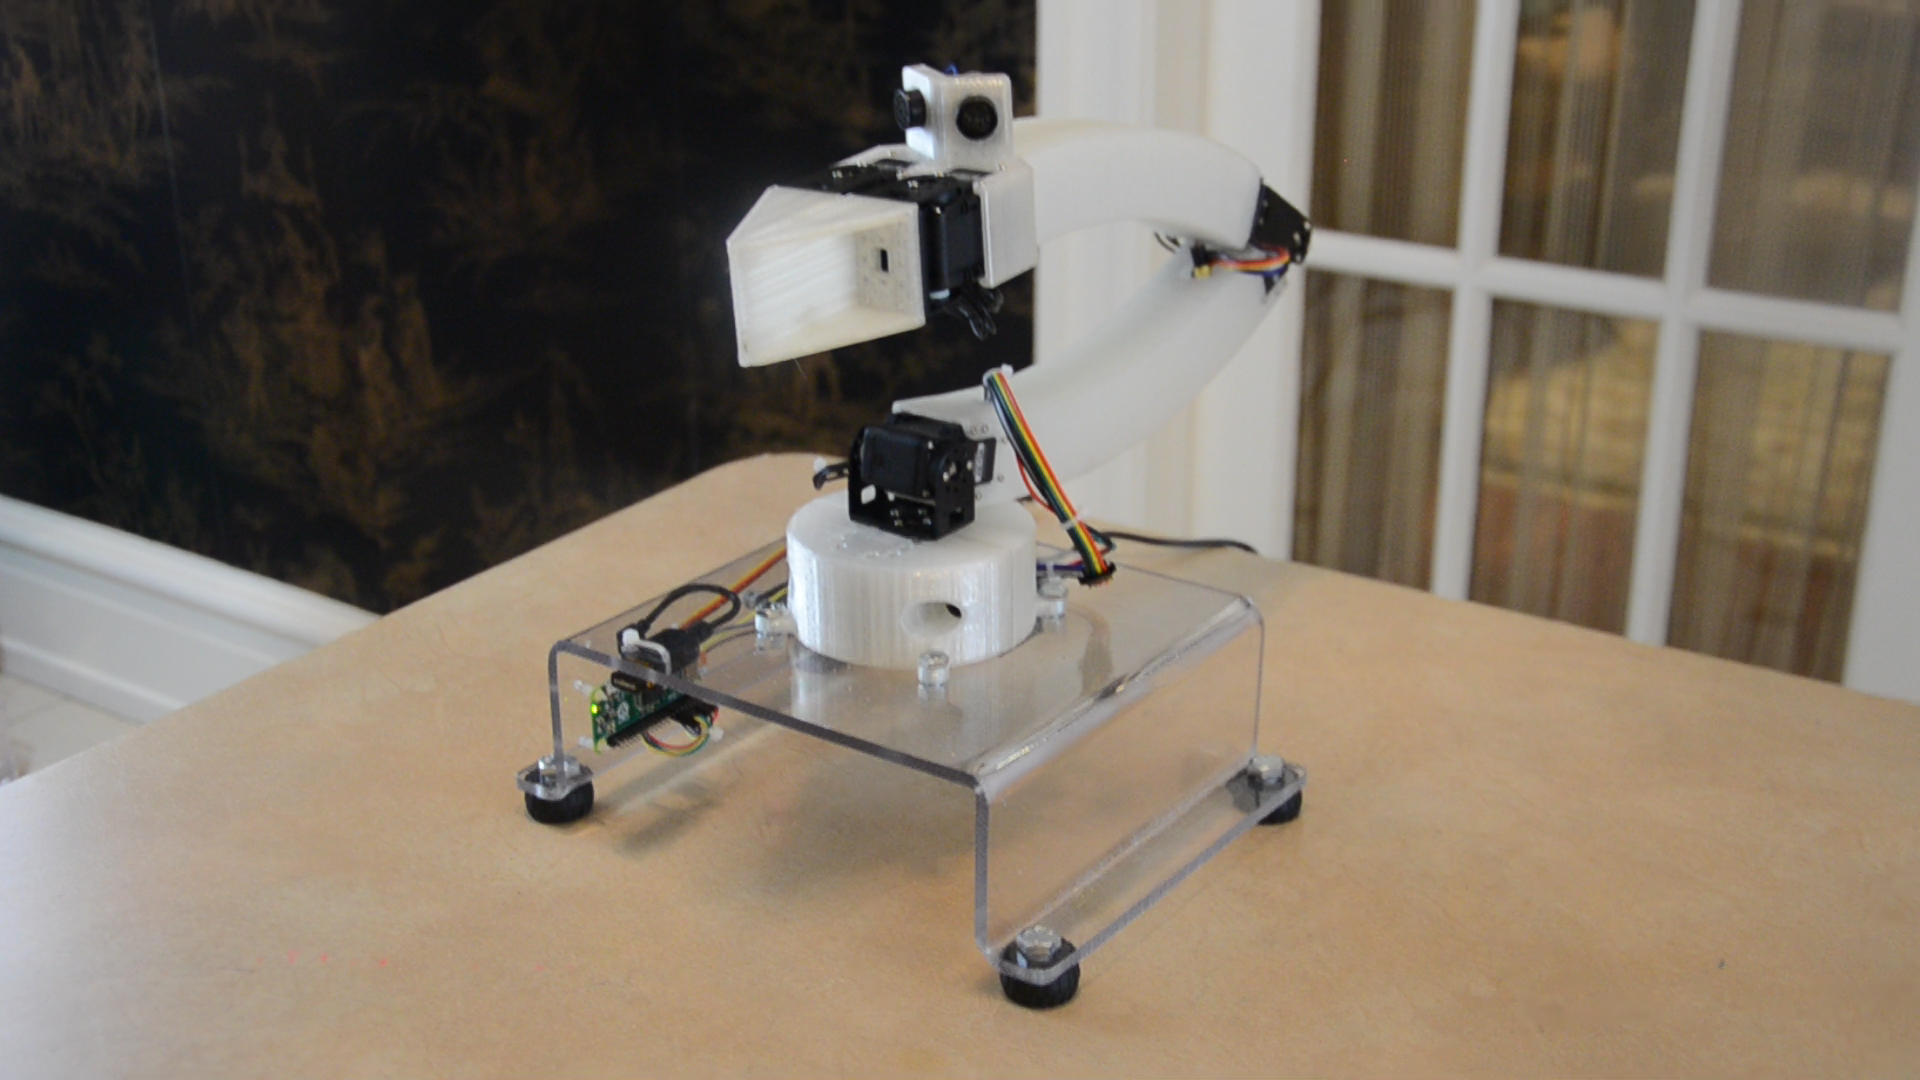
\includegraphics[height=6cm]{Figures/ThingThree.png}
	\caption{Fido Thing Three}
\end{figure}

The third and final hardware implementation constructed was a four axis robotic arm nicknamed ``Thing Three.''
A departure from the wheeled mobile robots previously detailled, Thing Three was created to demonstrate Fido's extensive universality and applicability in practical settings.
The robot's chassis was 3D printed out of translucent PLA plastic, with a hollow interior for wire and LED strip routing.
The LED strip was used to indicate reward administration during training.
The arm was actuated by five Dynamixel AX-12A servo motors, and controlled by a Raspberry Pi Zero.
The inputs to the system were two MaxSonar ultrasonic sensors and the arm's joints' current positions, while its outputs were its servo motors and LED strip.

\subsection{Training App}

\begin{figure}
	\centering
	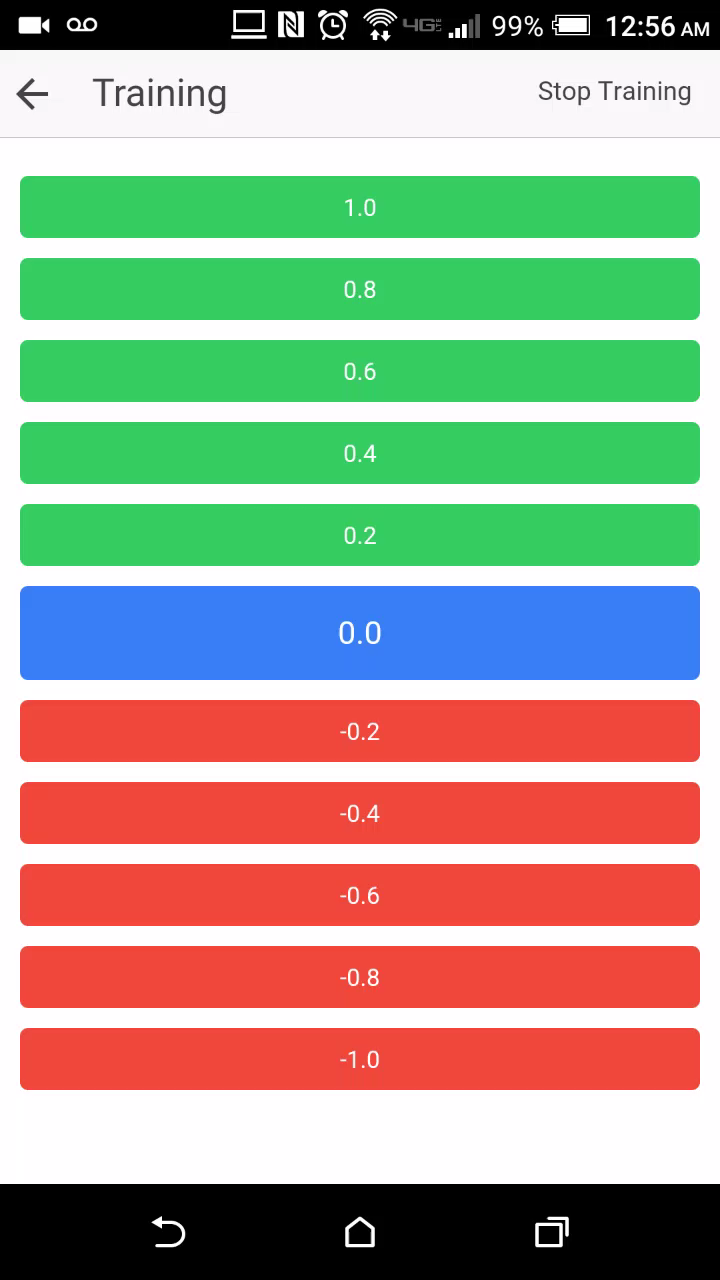
\includegraphics[height=6cm]{Figures/IonicScreenshot.png}
	\caption{Screenshot of the Training App during Robot Training}
\end{figure}

Next, a crossplatform mobile application was created to assist training Fido's hardware implementations.
The application allowed an operator to connect to a hardware implementation over Wi-Fi using TCP sockets, administer reward, and run trained models.
Gradient reward could be administered to the Fido control system from -1 to 1, with positive feedback shown in green and negative feedback shown in red.
The application was developed using web technologies through the Ionic Framework.


\section{Results}

\subsection{Results in Simulation}

To test Fido's effectiveness at learning with limited feedback, Fido was first trained on a number of different tasks through our simulator using reward values delegated through software.
Data was collected regarding Fido's latency and number of reward iterations needed for convergence.

Fido's first and simplest task, dubbed ``Flash,'' was to set the brightness value of an LED to a value proportional to the amount of light that Fido sensed.
Each reward iteration, Fido's neural network was given the intensity of visible light that Fido detected and was asked for the brightness value of Fido's LED.
Fido was then given a reward value equal to $1 - |b - v|$ where $b$ was the brightness value of Fido's LED ranging from 0 to 1 and $v$ was the intensity of visible light that Fido detected ranging from 0 to 1.

``Float,'' Fido's second task, challenged our learning implementation to direct a robot to point.
Each time it was told to select an action, Fido specified the robot's vertical and horizontal velocity between +30 and -30 pixels.
This emulates a holonomic drive systems, where motor outputs directly correlate to movement on the $x$ and $y$ axes.
At the start of each trial, Fido and the point were placed randomly on a boundless plane within 768 pixels of one another.
Fido was fed the ratio of its $x$ displacement to its $y$ displacement from its target point as the state.
Reward was calculated as the difference between Fido's distance away from the target point before performing the action and Fido's distance from the target point after performing the action.
Fido completed each trial when it was within 60 pixels of the point.

Fido's next task, nicknamed ``Drive,'' required that it direct a robot to point by controlling the motors of a differential drive system.
At the start of each trial, Fido and the point were placed randomly on a boundless plane within 768 pixels of one another.
Fido was fed the ratio of its $x$ displacement to its $y$ displacement from its target point as well as its rotation.
Reward was calculated as the difference between Fido's distance away from the target point before performing the action and Fido's distance from the target point after performing the action.
Fido completed each trial when it was within 60 pixels of the point.

Fido's last challenge, called ``Follow,'' was to perform the classic robotic task of line following by controlling the motors of the simulator's differential drive system.
At the start of each trial, Fido was placed on  a line with a random rotation.
Fido was fed the ratio of its $x$ displacement to its $y$ displacement from the closest point on the line as well as its rotation.
Reward was calculated as the difference between Fido's distance away from the line before performing the action and Fido's distance from the line after performing the action.
Fido completed each trial when it had stayed within 60 pixels of the line for 10 consecutive actions.

\subsubsection{Simulation Findings}

Each task was run 400 times to gather the data show in Table \ref{tab:data}.
The reward iterations values shown in the above data table were the medians of the data collected.
The median is shown instead of the mean to discount a few large outliers that were present in data.
The time data shown above is the mean of the data collected.

\begin{table}[ht]
	\centering
	\begin{tabular}{@{}lccc@{}}
		\toprule
		Task        & Learning Iterations & Action Selection (ms) & Training Time (ms) \\ \midrule
		Flash       & 6                   & 0.                 & 28                    \\
		Float       & 14                  & 1                  & 63                    \\
		Drive       & 16                  & 1                  & 94                    \\
		Line Follow & 10                  & 0.                 & 90.				   \\ \bottomrule
	\end{tabular}
	\caption{Number of Learning Iterations, Action Selection Time, and Training Time Per Iteration for Fido Simulation Tasks}
	\label{tab:data}
\end{table}

The data collected through the simulator demonstrates the prowess of the Fido control system with computer-delegated reward in multiple configurations and situations.
Fido was able to master both a holonomic and differential-drive motor control system (the ``Float'' and ``Drive'' tasks), proving its hardware agnostic capabilities.
All tasks showed low numbers of reward iterations and low latency, allowing Fido to learn quickly and efficiently.
The task that was most difficult for Fido, ``Drive,'' took a median of 16 reward iterations, well within the patience of a human.

\subsubsection{Comparison to Industry Standard of Q-Learning with a Neural Network}

Fido's performance in completing the above simulator tasks was tested against the industry standard of discrete Q-Learning using a neural network.  On average, Fido required \textbf{over four times fewer} learning iterations than discrete Q-Learning for a given task.

\begin{table}[ht]
	\centering
	\small
		\begin{tabular}{lYY}
			\toprule
		Task        & Fido Learning Iterations & Discrete Learning Iterations \\ \midrule
			Flash             & 3   & 16  \\
		Float to Point    & 14  & 56  \\
		Drive to Point    & 16  & 69  \\
			Line Following    & 10  & 42 \\
		\caption {Fido Results Compared to Discrete Q-Learning}
			\label{tab:simindustrystandardresults}
	\end{tabular}
\end{table}

\subsection{Results in Hardware}

Data was next collected from Fido's hardware implementations to gage performance with human given feedback in real world situations.
Reward was administered through the mobile application previously discussed.  25 trials were done for each task to gather the data shown in the below tables.  As with the simulation, reward iterations values shown are the medians of the data collected while time data shown is the mean of the data collected.

\subsubsection{Thing One Results}

The first task to be given to Thing One was to stay still.
As one would expect, Fido's sole responsibility for this task was not to move.
Fido was administered positive reward when it didn't move, and negative reward when it did.
Next, Thing One was tasked with driving to a point.
At the start of each trial, Fido and the point were placed randomly on a smooth, hardwood surface within 0.75 meters of one another.
Fido was told the ratio of its $x$ displacement to its $y$ displacement from its target point as well as its rotation.
Every fourth action that Fido made was chosen as a reward iteration, and Fido was given a reward value corresponding to its last action.
This reward value was chosen by the tester based on whether Fido moved toward the point or not.
Fido completed each trial when it was within 10 cm of the point.


\begin{table}[ht]
	\centering
	\begin{tabular}{@{}lccc@{}}
		\toprule
		Task             & Learning Iterations & Action Selection (ms) & Training Time (ms) \\ \midrule
		Stay Still       & 3                   & 1                    & 43.5                  \\
		Drive to Point   & 18                  & 4                     & 65                  \\
	\end{tabular}
	\caption{Number of Learning Iterations, Action Selection Time, and Training Time Per Iteration for Thing One Tasks}
	\label{tab:data2}
\end{table}

Performance was slower on the hardware implementation than in simulation for the drive to point task due to the limited computation power of the Intel Edison compute model compared to modern desktop computers.
However, the results still demonstrated Fido's real world applicability through its ability to perform outside of a simulation environment.

\subsubsection{Thing Two Results}

The second hardware implementation constructed, nicknamed ``Thing Two,'' was tasked to master its complex holonomic drive system and numerous sensors to master tasks with limited preprocessing.
The first task administered asked Fido to drive straight using its three 90$^{\circ}$ Swedish wheels, requiring Fido to determinethe correct ratio of motor values outputted.
Fido was administered reward somewhat subjectively by a human operator, being given positive reward when it drove in a less lopsided fashion.
Next, Fido was tasked with following a line.
Fido's line sensor reported whether it was to the left or right of a line.
A course was laid out using black electrical tape for Thing Two to learn on.
Training was performed by placing Thing Two to the left or right of a line.
If the robot moved towards the line, it was administered positive feedback.
If the robot moved away from the line, it would receive negative feedback.
Fido was also trained to follow a ball using its ZX sensor, which reported the location of an object in front of it in the horizontal and vertical dimensions.
Similiarly, Fido was administered positive reward if it drove towards the ball, and negative reward if it drove away.
Finally, Fido's retrainability and applicability was tested in a task that involved loading a pretrained line following model, unplugging a motor, and retraining the robot to compensate.

\begin{table}[ht]
	\centering
	\begin{tabular}{@{}lccc@{}}
		\toprule
		Task              & Learning Iterations & Action Selection (ms) & Training Time (ms) \\ \midrule
		Drive Straight         & 13             & 2                     & 215                \\
		Line Following         & 15             & 21                    & 398                \\
		Fetch                  & 8              & 1                     & 246                \\
		Limping Line Following & 6              & 20                    & 464                \\ \bottomrule
	\end{tabular}
	\caption {Number of Learning Iterations, Action Selection Time, and Training Time Per Iteration for Thing Two Tasks} \label{tab:thingtworesults}
\end{table}

\subsubsection{Thing Three Results}

The last hardware implementation constructed was a four axis robotic arm, nicknamed ``Thing Three.''
Thing Three was first tasked with drawing a square.
As output, Fido could choose from a set of ``waypoints,'' predefined sets of angle positions representing important positions in the operating enviroment.
As input, Fido was given its current waypoint.
If Fido drew a correct line in the sequence of drawing a square, it was given positive reward.
Next, Thing Three was trained to hit a ball with a paddle (or ``play ping pong'') using its two ultrasonic sensors to sense ball position.
Fido was able to adjust its joint rotations as outputs to hit the ball.
In training, positive feedback was administered if Thing Three hit the paddle towards the ball, while negative feedback was given if Thing Three moved in the opposite direction.

\begin{table}[ht]
	\centering
	\begin{tabular}{@{}lccc@{}}
		\toprule
		Task              & Learning Iterations & Action Selection (ms) & Training Time (ms) \\ \midrule
		Draw Square         & 5                   & 5                    & 40                 \\
		Ping Pong          & 8                  & 3                    & 379                \\
		\bottomrule
	\end{tabular}
	\caption {Number of Learning Iterations, Action Selection Time, and Training Time Per Iteration for Thing Three Tasks} \label{tab:thingthreeresults}
\end{table}


\section{Conclusion}

A general robotic control system nicknamed Fido was developed that learned tasks with limited feedback.
Fido couples the training of artificial neural networks with a wire-fitted moving least squares interpolator to achieve a continuous state-action space $Q$-learning reinforcement algorithm implementation.
Fido leverages a Boltzmann distribution of probability based on reward to select actions, allowing it to continuously explore its state-action space.
A kinematically accurate robot was simulated with a differential drive system, a sensor array, and other outputs for testing and evaluation purposes.
The robot was trained on a number of common robotic tasks and successfully converged on these tasks in very few learning iterations while maintaining impressively low latency.
Next a hardware implementation was built using a differential drive system, capable of utilizing real world sensor inputs to learn tasks such as driving to a point and staying still.
In the future, we hope to further improve Fido's software and consider further applications in the present.


\nocite{gaskett,geoffrey,werbos,dini,macleod,dongsoo,dudek,watkins,rummery,baird}

\pagebreak
\bibliography{Paper}
\bibliographystyle{apacite}

\end{document}
